\chapter{$ISA^{2}$}

Hemos hablado en la introducción sobre las soluciones \ac{ISA} a grandes rasgos y la principal novedad de $ISA^{2}$ frente a éstas. En este capítulo vamos a comenzar revisando el estado del arte (Sección \ref{sec:isa2_estado_del_arte}, destacando trabajos relacionados en el ámbito de las soluciones \ac{ISA}. Finalmente, en la Sección \ref{isa2_model}, detallaremos el sistema $ISA^{2}$ sobre el que hemos trabajado en este proyecto.


\section{Trabajos relacionados}
\label{sec:isa2_estado_del_arte}
%TODO: Añadir una revisión del estado del arte en tecnología ISA. Describir primero soluciones comerciales, y cómo funcionan. Luego añadir otro párrafo de soluciones que se basen en imágenes o que sean papers que soluiones el problema. Puedes traducir y reescibir de nuevo la sección del estado del arte del paper de ISA^2.

\section{El modelo $ISA^{2}$}
\label{isa2_model}

Para poder explicar la metodología, antes debemos de preguntarnos cómo funciona todo el sistema de $ISA^{2}$, centrándonos en cada parte que lo compone para que resulte más fácil su comprensión. He aquí unas figuras ilustrativas que nos servirán como punto de referencia durante todo el capítulo:


\begin{figure}[H]
  \centering
  \includegraphics[width=8cm]{Figuras/Figura_Esquema_ISA2_Version_1_SegSem.eps}
  \caption{Esquema $ISA^{2}$ Antiguo}
  \label{fig:Isa_v1}
\end{figure}


Como se puede ver al pie de la figura \ref{fig:Isa_v1}, este fue el esquema utilizado para la primera versión de $ISA^{2}$ \cite{isa2} y funcionaba de la siguiente manera:


\begin{itemize}
\item En primera instancia el sistema recogía un set de imágenes que se correspondía con situaciones de tráfico tanto en autovía (o autopista) como en núcleos urbanos. Cuando el sistema tenía que procesar una imagen, ésta venía en diferentes escalas puesto que el modelo de \textbf{DeepLab} de \ac{SS} trabajaba así. Este modelo tenía como base una \ac{CNN}, es decir, una \textbf{Red Neuronal Convolucional} \cite{cnn}.
 
\item Este tipo de tecnología es la que posibilitó entonces, y ahora, la \ac{SS} de las imágenes.

\item Tras este proceso, mediante unos códigos de \textbf{Matlab} se recogían los datos de los píxeles ya segmentados y se organizaban en histogramas. Basándonos en los histogramas generados, usábamos una estrategia llamada \ac{SPP} \cite{spp} para crear un descriptor de imagen.

\item Por último, el descriptor generado en el paso anterior se pasaba a diferentes sistemas de regresión. Para cada uno de ellos se añadía \ac{SI} \cite{spp} usando \ac{SPP} de hasta 3 niveles para poder compararlos entre sí y saber cuál era mejor. Para ello cogíamos los mejores resultados de cada sistema entre todos los niveles usados, y los usábamos como referencia.

\end{itemize}

\subsection{Segmentación Semántica}

Pero, ¿qué es la \ac{SS}? ¿Y por qué es tan útil en este proyecto?

En el capítulo anterior hablamos de una forma resumida en qué consiste la \ac{SS} y su uso en el proyecto, pero es tan solo la punta del iceberg.


La \ac{SS} es un proceso por el cual los píxeles de una imagen son dotados de distintos valores para poder diferenciarlos en etiquetas unos de otros y así reconocer los elementos que componen dicha imagen \cite{deeplab}. 

Por ejemplo: Una fotografía de una persona, un coche y un perro. A priori, todos los píxeles de la imagen no están categorizados y no se sabe qué partes de la imagen corresponden a la persona, al coche, y al perro. Gracias a la segmentación semántica los píxeles de la imagen adquieren los valores de las etiquetas referentes a \textbf{persona}, a \textbf{coche} y a \textbf{perro}; y son fácilmente distinguibles entre sí.

Más adelante usaremos unos códigos en MatLab que trabajan con estas etiquetas para generar los histogramas.

\subsection{mIoU}

Para saber qué porcentaje de acierto ha tenido el proceso nos basaremos en la \ac{mIoU} \cite{miou-iou}. Esta métrica se basa en hacer la media de la \ac{IoU} de las diferentes etiquetas de clases.

La \ac{IoU} \cite{miou-iou} es la relación de superposición que existe entre la imagen segmentada y la original. Es decir, sirve para dictaminar con cuánta precisión se ha realizado el proceso de \ac{SS}. En las siguientes figuras se puede ver un ejemplo muy práctico:

\begin{figure}[H]
  \centering
  \includegraphics[width=8cm]{Figuras/Iou_1.eps}
  \caption{Imagen Original}
\end{figure}

\begin{figure}[H]
  \centering
  \includegraphics[width=8cm]{Figuras/IoU_2.eps}
  \caption{Predicción}
\end{figure}


Fue de esta manera como se pudo ejecutar con eficacia este sistema \cite{isa2}. Sin embargo, con el paso de los años surgieron nuevos modelos de \ac{SS} más eficaces y precisos, y fruto de ello es el sistema que hemos utilizado en esta nueva versión: \textbf{Swiftnet} \cite{swiftnet}.


\begin{figure}[H]
  \centering
  \includegraphics[width=8cm]{Figuras/Figura_Esquema_ISA2_Version_2.eps}
  \caption{Esquema $ISA^{2}$ Actual}
    \label{fig:Isa_v2}
\end{figure}


Como se puede comprobar, el esquema de la figura \ref{fig:Isa_v2} sigue el mismo camino que el de la primera versión, salvo por unas modificaciones al principio que pasamos a explicar a continuación:

\begin{enumerate}

\item Las imágenes de entrada al modelo de \ac{SS} no llegan en diferentes escalas como se podría intuir. La razón de por qué es así es Swiftnet: El modelo admite tanto imágenes en diferentes escalas como imágenes con una única escala.


Sin embargo, para este proyecto hemos optado por la recomendación de los autores \cite{github_swiftnet} y hemos decidido hacerlo con una única escala. De esta manera hemos obtenido los resultados esperados con la base de datos de \textbf{Cityscapes} \cite{cityscapes} que ellos mismos utilizaron \cite{swiftnet}.

\item La segunda, y última, modificación es la más obvia: la sustitución del modelo de DeepLab \cite{deeplab} por el modelo de Swiftnet \cite{swiftnet}.

A diferencia del primero, Swiftnet es un modelo que opera en tiempo real (\textbf{Real-Time}) de tal modo que cuando procesa una imagen lo hace en el momento, mientras que DeepLab tiene que esperar a que se recoja un set de imágenes para luego ir procesándolas.

\end{enumerate}


En el siguiente capítulo hablaremos acerca de la implementación de Swiftnet y de cómo es mejor para los campos de aplicación, especificados anteriormente, con respecto a DeepLab.
